\documentclass[12pt,a4paper]{article}%
\usepackage[]{graphicx}\usepackage[]{color}
%% maxwidth is the original width if it is less than linewidth
%% otherwise use linewidth (to make sure the graphics do not exceed the margin)

%2multibyte Version: 5.50.0.2960 CodePage: 1252
\usepackage{amsfonts}
\usepackage{amssymb}
\usepackage[centertags]{amsmath}
\usepackage{graphicx}%
\usepackage{natbib}
\usepackage{color}
\usepackage[dvipsnames,svgnames*]{xcolor}
\usepackage{array}
\usepackage[hidelinks]{hyperref}
\usepackage[font=small,skip=5pt]{caption}
\usepackage[aboveskip=2pt]{subcaption}
\usepackage{amsmath}
\usepackage[]{algorithm2e}
\usepackage{amsthm}
\usepackage{url}
\usepackage{wasysym}
\usepackage{ulem}
\usepackage{afterpage}
\usepackage{bbm}
\setcounter{MaxMatrixCols}{30}
\providecommand{\U}[1]{\protect\rule{.1in}{.1in}}
\newtheorem{theorem}{Theorem}
\newtheorem{acknowledgement}[theorem]{Acknowledgement}
\newtheorem{axiom}[theorem]{Axiom}
\newtheorem{case}[theorem]{Case}
\newtheorem{claim}[theorem]{Claim}
\newtheorem{conclusion}[theorem]{Conclusion}
\newtheorem{condition}[theorem]{Condition}
\newtheorem{conjecture}[theorem]{Conjecture}
\newtheorem{corollary}[theorem]{Corollary}
\newtheorem{criterion}[theorem]{Criterion}
\newtheorem{definition}[theorem]{Definition}
\newtheorem{example}[theorem]{Example}
\newtheorem{exercise}[theorem]{Exercise}
\newtheorem{lemma}[theorem]{Lemma}
\newtheorem{notation}[theorem]{Notation}
\newtheorem{problem}[theorem]{Problem}
\newtheorem{proposition}[theorem]{Proposition}
\newtheorem{remark}[theorem]{Remark}
\newtheorem{solution}[theorem]{Solution}
\newtheorem{summary}[theorem]{Summary}
\setlength{\topmargin}{0in}
\setlength{\oddsidemargin}{0.1in}
\setlength{\evensidemargin}{0.1in}
\setlength{\textwidth}{6.5in}
\setlength{\textheight}{8.25in}
\numberwithin{equation}{section}
\title{Real Time Variational Density Forecasting}
\author{Nathaniel Tomasetti}
\begin{document}

\maketitle
\tableofcontents
\section{Introduction} \label{sec:Intro}

Electricity prices have been the subject of an extensive forecasting literature and are known to be extremely volatile. For the 2011-2015 period in Victoria the mean price per megawatt hour (mWh) was \$42.06, with 99\% of observations less than \$100 per mWh, however on several occasions the price spiked to greater than $10,000\%$ of the mean value. For this reason market participants are increasingly interested in a predictive density forecast, as the probability that the price will rise above a particular threshold in the next time period can be more important than the mean value. To calculate a suitably accurate predictive density the Bayesian methodology is to be adopted in this thesis, as it accounts for both parameter and model uncertainty in a relatively straightforward manner, which can be difficult in frequentist methods. See \citet{Geweke2006} for a review on Bayesian forecasting and \citet{Gneiting2014} for a discussion of density forecasting in general. 

Bayesian methods are computationally complex as they require integration over the set of unknowns, whether parameters or latent stochastic variables. This set is typically quite large for models used to model short term electricity load and price as there are strong seasonal patterns in the data \citep{Taylor2003}. Analytical integration is typically not feasible to obtain the predictive distribution for such models, however there are a range of numerical and simulation-based techniques available for this purpose, notably Markov Chain Monte Carlo (MCMC) methods. While it is often possible to demonstrate theoretical convergence of MCMC algorithms, computation may be slow for even moderately complex models. This is problematic when attempting to forecast electricity load in Victoria, as realizations occur at five minute intervals, making it difficult to compute the predictive density for the next period's electricity load within the time frame.

Alternatives to MCMC include Variational Bayes (VB) methods, where the aim is to replace the unknown true posterior distribution for a vector of unknowns with a parametric approximation. The Variational Bayes approach will be explored in the thesis, to determine if it is a viable alternative computation strategy to MCMC, in the context of modelling and short term forecasting of Victorian electricity load. In particular, we seek to understand the benefits gained in terms of the computational time required to obtain a VB approximate forecast distribution against the loss in statistical accuracy associated with the use of an approximate posterior forecast distribution. 

The literature on Variational Bayes is dominated by two major implementations: Mean Field Variational Bayes (MFVB) and what we call Stochastic Variational Bayes (SVB). For either implementation we emphasise that there are two seperate tasks: Choose a functional form for the approximating distribution, and then optimise the parameters of this distribution to minimise a well defined divergence between the approximation and the true posterior. A recent review of Variational Bayes is provided by \citet{Blei2017}.

Mean Field Variational Bayes (see \citet{Bishop2006} for an overview) can be applied to exponetial family models with conjugate priors, and restricts the class of approximating distributions to the factorisable family. MFVB provides both the optimal form of the approximating distribution within this class, and a computationally simple coordinate ascent algorithm to optimise parameters.
Stochastic Variational Bayes (see \citet{Paisley2012} and \citet{Ranganath2014}) lifts both the restrictions for an exponential family model and the use of an approximating distribution that is factorisable. While parameter optimisation has a well developed gradient ascent algorithm, the determination of the functional form to be used is an active area of research.

We explore the use of a copula to augment the approximating distribution with a flexible dependence structure, which has seen success in \citet{Tran2015} and \citet{Ng2016}. The time series context of our implementation implies that MCMC samples for out of date samples are available, and we exploit this information in the construction of a vine copula so that the approximation has a dependence structure similiar to the true posterior. 

The discussion of MCMC and VB will be continued in Section \ref{sec:BayesInf}, with the methods contrasted in the context of two simple models. Section \ref{sec:ElecLoad} will introduce a planned empirical application of VB to Victorian electricity load using an exponential smoothing model and data from the 2012-2015 period. Section \ref{sec:Discussion} outlines the major areas to which this thesis will make a contribution, and Section \ref{sec:Timeline} outlines the planned timeline for these contributions.

\section{Bayesian Inference} \label{sec:BayesInf}

To facilitate the discussion, consideration is given to models where the unknowns may be summarized in a (finite) $k-$dimensional vector, denoted by $\boldsymbol{\theta}.$ In this setting, given an observed time series, denoted by $y_{1:T}= \{y_{t}, t = 1, \dots T\}$, the Bayesian forecast distribution associated with time $t=T+1$ is characterized by the conditional density
\begin{equation}
\label{predictive}
p(y_{T+1} | y_{1:T}) =\int p(y_{T+1}|y_{1:T},\boldsymbol{\theta}) p(\boldsymbol{\theta}|y_{1:T}) d\boldsymbol{\theta},
\end{equation}
where $p(\boldsymbol{\theta}|y_{1:T})$ denotes the posterior density for $\boldsymbol{\theta}$, given by
\begin{equation}
\label{posterior}
 p(\boldsymbol{\theta} | y_{1:T}) = \frac{p(y_{1:T}|\boldsymbol{\theta})p(\boldsymbol{\theta})}{\int p(y_{1:T}|\boldsymbol{\theta})p(\boldsymbol{\theta}) d\boldsymbol{\theta}}.
\end{equation}

Generally the analytical solution to (\ref{posterior}), and hence to (\ref{predictive}) will be unavailable due to the complex functional form of the distributions involved. 
In this section two alternative methods for computing the desired posterior distribution in (\ref{posterior}),  MCMC and VB, will be reviewed.
In brief, MCMC is used to create a sample from $p(\boldsymbol{\theta} | y_{1:T})$, with any function of $\boldsymbol{\theta}$ that is desired estimated from that sample. In contrast, VB replaces $p(\boldsymbol{\theta} | y_{1:T})$ with an approximation, denoted by $q(\boldsymbol{\theta} | \boldsymbol{\lambda})$, where $\boldsymbol{\lambda}$ is a vector of auxiliary parameters associated with the approximation that may depend on the observations $y_{1:T}$.
For example, if $q(\boldsymbol{\theta} | \boldsymbol{\lambda})$ is Gaussian, then $\boldsymbol{\lambda}$ would denote the mean and variance parameters that characterise this distribution for $\boldsymbol{\theta}$.  Variational Bayes aims to choose the distribution $q(\boldsymbol{\theta} | \boldsymbol{\lambda})$ within a restricted class such that the a measure of divergence, typically the Kullback-Leibler divergence from $q(\boldsymbol{\theta} | \boldsymbol{\lambda})$ to $p(\boldsymbol{\theta} | y_{1:T})$, is minimised. Once the posterior distribution in (\ref{posterior}) is available, the predictive density forecast (\ref{predictive}) can be found by simulation.

\subsection{Markov Chain Monte Carlo} \label{sec:MCMC}

There are many types of MCMC algorithms, with arguably the simplest and most commonly used one being the Gibbs sampler. The Gibbs sampler algorithm iteratively samples the components of the $k-$dimensional parameter vector $\boldsymbol{\theta}$ via each of the so-called full conditional distributions as follows,
\begin{align}
&p(\theta_1 | \theta_2, \dots, \theta_k, y_{1:T}) \nonumber \\
&p(\theta_2 | \theta_1, \theta_3, \dots, \theta_k, y_{1:T}) \nonumber \\
&\vdots \nonumber \\
&p(\theta_k | \theta_1, \dots, \theta_{k-1}, y_{1:T}). \nonumber
\end{align}
Under mild regularity conditions (see, e.g., \citet{Tierney1994}) and with enough iterations of the Markov chain that results from the Gibbs sampler, these samples converge in distribution to $p(\boldsymbol{\theta} | y_{1:T})$. Samples taken before the MCMC converges to the posterior must be discarded, and the remaining samples may have strong dependence between consecutive draws of the same parameter due to the Markov nature of the algorithm. The computation time for each iteration and the overall number of iterations required to accruately summarise the posterior distribution is problem specific and typically increases with the number of parameters in the model. On occasion, the full conditional distribution cannot be recognised and a Metropolis-Hastings-within-Gibbs step can be used, see \citet{Gilks1995} for details.

For illustration, consider data $y_t$ for $t = 1, \dots, T$ generated independently from a $\mathcal{N}(\mu, \sigma^2)$ distribution with prior distributions given by $\mu | \sigma^2 \sim \mathcal{N}(\gamma, \sigma^2/\tau)$ and $\sigma^2 \sim IG(\mbox{shape} = \alpha, \mbox{scale =}\beta)$, where $IG$ repesents the inverse of a Gamma distribution. It can be shown that

\begin{align}
&\mu | \sigma^2, y_{1:T} \sim \mathcal{N} \left(\frac{\tau\gamma + T\bar{y}}{\tau + T}, \frac{\sigma^2}{\tau  + T} \right) \label{posmu} \\
&\sigma^2 | \mu, y_{1:T} \sim IG  \left( \mbox{shape} = \alpha + T/2, \mbox{scale} = \beta + \frac{1}{2}\sum_{t=1}^{T}y_t^2 + \tau\gamma^2 - \frac{(\tau\gamma + T\bar{y})^2}{\tau + T} \right) \label{possig2} 
\end{align}
where $\bar{y} = 1/T \sum_{t=1}^{T}y_t$. Posterior sampling can proceed by first simulating $\sigma^2$ from (\ref{possig2}) and conditioning on this draw to simulate $\mu$ from (\ref{posmu}).

\subsection{Variational Bayes} \label{sec:VB}

As discussed in Section \ref{sec:Intro}, a faster (albeit approximate) alternative to MCMC is VB. VB is an umbrella term for a broad collection of algorithms that introduce an approximating distribution $q(\boldsymbol{\theta} | \boldsymbol{\lambda})$ with the choice of the functional form $q$ and subsequent auxiliary parameter vector $\boldsymbol{\lambda}$ determined so that an error function is minimised. The classical choice for this error function is the Kullback-Leibler (KL) divergence \citep{Kullback1951} from $q(\boldsymbol{\theta} | \boldsymbol{\lambda})$ the true posterior $p(\boldsymbol{\theta} | y_{1:T})$. The KL divergence is defined by
\begin{equation}
\label{KL-def}
KL[q(\boldsymbol{\theta} | \boldsymbol{\lambda})\hspace{.1cm}||\hspace{.1cm}p(\boldsymbol{\theta} | y_{1:T})] = \int q(\boldsymbol{\theta} | \boldsymbol{\lambda}) \ln \left( \frac{q(\boldsymbol{\theta} | \boldsymbol{\lambda})}{p(\boldsymbol{\theta} |y_{1:T})}\right) d\boldsymbol{\theta}.
\end{equation}
The KL divergence is a non-negative, asymmetric measure of the discrepancy between $p(\boldsymbol{\theta} | y_{1:T})$ and $q(\boldsymbol{\theta} | \boldsymbol{\lambda})$  that will be equal to zero if and only if $p(\boldsymbol{\theta} | y_{1:T}) = q(\boldsymbol{\theta} | \boldsymbol{\lambda})$ almost everywhere \citep{Bishop2006}. Note that $KL[q(\boldsymbol{\theta} | \boldsymbol{\lambda})\hspace{.1cm}||\hspace{.1cm}p(\boldsymbol{\theta} | y_{1:T})]$ can be expressed as
\begin{equation}
\label{KL-ELBO}
KL[q(\boldsymbol{\theta} | \boldsymbol{\lambda})\hspace{.1cm}||\hspace{.1cm}p(\boldsymbol{\theta} | y_{1:T})] = \ln(p(y_{1:T})) - \mathcal{L}(q(\boldsymbol{\theta} | \boldsymbol{\lambda}), y_{1:T})
\end{equation}
where $\mathcal{L}(q(\boldsymbol{\theta} | \boldsymbol{\lambda}), y_{1:T})$ is referred to as the Evidence Lower Bound (ELBO), as it provides a lower bound on the unknown constant $\ln(p(y_{1:T}))$.  $\mathcal{L}(q(\boldsymbol{\theta} | \boldsymbol{\lambda}), y_{1:T})$ is defined by
\begin{equation}
\label{ELBO}
\mathcal{L}(q(\boldsymbol{\theta} | \boldsymbol{\lambda}), y_{1:T}) = \int q(\boldsymbol{\theta} | \boldsymbol{\lambda}) \ln (p(y_{1:T},\boldsymbol{\theta})) d\boldsymbol{\theta} -  \int q(\boldsymbol{\theta} | \boldsymbol{\lambda}) \ln (q(\boldsymbol{\theta} | \boldsymbol{\lambda})) d\boldsymbol{\theta}.
\end{equation}

Since $\ln(p(y_{1:T}))$ is constant with respect to $q(\boldsymbol{\theta} | \boldsymbol{\lambda})$, maximising (\ref{ELBO}) with respect to $q(\boldsymbol{\theta} | \boldsymbol{\lambda})$ is equivalent to minimising (\ref{KL-def}). Maximising the ELBO is much more convenient than minimising the KL Divergence, as will be shown in the following sections in the context of the two major implementations of Variational Bayes we consider, Mean Field Variational Bayes and Stochastic Variational Bayes. Each of these implementations takes advantage of the functional form of the ELBO, and offers a computationally efficient algorithm to for finding $q(\boldsymbol{\theta} | \boldsymbol{\lambda})$ that is optimal within a particular class of distributions. The statistical properties of $q(\boldsymbol{\theta} | \boldsymbol{\lambda})$ in MFVB and SVB are largely driven by the choice of the KL divergence from $q(\boldsymbol{\theta} | \boldsymbol{\lambda})$ to $p(\boldsymbol{\theta} | y_{1:T})$ as an error function, and there is significant interest in other error functions, such as the KL divergence from $p(\boldsymbol{\theta} | y_{1:T})$ to $q(\boldsymbol{\theta} | \boldsymbol{\lambda})$ \citep{Minka2001} and Stein's discrepency (\citealp{Liu2016}; \citealp{Ranganath2016b}).

\subsubsection{Mean Field Variational Bayes} \label{sec:mfvb}

Mean Field Variational Bayes (MFVB) has its origin in physics \citep{Peterson1987} and has since developed a large literature in machine learning, notably \citet{Jordan1999} and \citet{Ghahramani2000}. MFVB restricts the class of distributions from which to select $q(\boldsymbol{\theta} | \boldsymbol{\lambda})$ to the set of factorisable distributions,
\begin{equation}
\label{mf1}
q(\boldsymbol{\theta} | \boldsymbol{\lambda}) = \prod_{i=1}^k q_i(\theta_i | \boldsymbol{\lambda_i}).
\end{equation}

The $k$ components $\theta_i$ may be a vector, but in most implementations are scalars. Each $\theta_i$ has an associated vector $\boldsymbol{\lambda_i}$ that may have a different dimension from $\theta_i$. $\boldsymbol{\lambda_i}$ is an auxillary parameter vector for the relevant factor $q_i$, which will be used in this section as shorthand notation for the distribution $q_i(\theta_i |\boldsymbol{\lambda_i})$. 

MFVB is widely used as it greatly simplifies maximisation of the ELBO, and has a straight-forward implementation in exponential family models \citep{Wainwright2008}.  Maximising the ELBO with respect to $q_i$ is as analytically involved as deriving the conditional distributions used in Gibbs based MCMC schemes, but the resulting algorithm to maximise the ELBO is much simpler computationally than sampling from a Gibbs MCMC scheme. MFVB factorises (\ref{ELBO}) into a product of $k$ separate components that each contain only one $q_i$, and then maximises each of these factors with respect to the associated $q_i$. Using the notation $q_{\setminus i} = \prod_{j\neq i}q_j$, \citet{Attias1999} shows that each component is maximised by
\begin{equation}
\label{mf2}
q_i(\theta_i |\boldsymbol{\lambda_i}) \propto\exp( \mathbb{E}_{q_{\setminus i}} [\ln(p(y_{1:T},\boldsymbol{\theta}))]).
\end{equation}

We illustrate the implementation of MFVB with the model considered in Section (\ref{sec:MCMC}), where $y_t$ for $t = 1, \dots, T$ is generated independently from a $\mathcal{N}(\mu, \sigma^2)$ distribution, and prior distributions are given by $\mu \sim \mathcal{N}(\gamma, \sigma^2 / \tau)$ and $\sigma^2 \sim IG(\mbox{shape} = \alpha, \mbox{scale =}\beta)$. It can be shown that
\begin{equation}
\label{mf3}
q(\mu | \boldsymbol{\lambda}_1) \propto \exp \left\{ \frac{-(T + \tau) \mathbb{E}_{q(\sigma^2)}[\sigma^{-2}]}{2} \left( \mu - \frac{\tau \gamma + \sum_{t=1}^{T} y_t}{T + \tau} \right)^2 \right\}
\end{equation}
and
\begin{align}
\label{mf4}
q(\sigma^2 | \boldsymbol{\lambda}_2) &\propto \sigma^{-2((T+1)/2 + \alpha + 1)} \nonumber \\
\times &\exp \left\{ \frac{ \beta + 1/2\left((\tau + T)\mathbb{E}_{q(\mu)}[\mu^2] - 2 \mathbb{E}_{q(\mu)}[\mu ]\left(\sum_{t=1}^{T}y_t + \tau \right) + \sum_{t=1}^{T} y_t^2 + \tau \gamma^2\right)}{-\sigma^2} \right\}.
\end{align}

As the prior distributions used were conjugate to the likelihood, the Variational Bayes optimal distributions for $q(\mu |  \boldsymbol{\lambda}_1)$ and $q(\sigma^2 | \boldsymbol{\lambda}_2)$ are the same family as the prior distributions, and are denoted by $q(\mu | \boldsymbol{\lambda}_1) \sim \mathcal{N}(\tilde{\gamma}, \tilde{\tau})$ and $q(\sigma^2 | \boldsymbol{\lambda}_2) \sim IG(\tilde{\alpha}, \tilde{\beta})$. The vector $\boldsymbol{\lambda} = (\tilde{\gamma}, \tilde{\tau}, \tilde{\alpha}, \tilde{\beta})'$ is given by
\begin{align}
\tilde{\gamma} &= \frac{\tau \gamma + \sum_{t=1}^{T} y_t}{T + \tau}  \label{mf5} \\ 
\tilde{\tau} &= \left((T + \tau)\mathbb{E}_{q(\sigma^2)}[\sigma^{-2}]\right )^{-1} \label{mf6} \\
\tilde{\alpha} &= (T+1)/2 + \alpha  \label{mf7} \\
\tilde{\beta} &= \beta + 1/2\left((\tau + T)\mathbb{E}_{q(\mu)}[\mu^2 ]- 2 \mathbb{E}_{q(\mu)}[\mu ]\left(\sum_{t=1}^{T}y_t + \tau\right) + \sum_{t=1}^{T} y_t^2 + \tau \gamma^2 \right). \label{mf8}
\end{align}.

The expectations in (\ref{mf5}) - (\ref{mf8}) are available in a closed form for these distributions, and these are substituted into (\ref{mf6}) and (\ref{mf8}) to yield the set of mean field equations:
\begin{align}
\tilde{\tau} &= \frac{\tilde{\beta}}{\tilde{\alpha}(T + \tau)} \label{mf9} \\
\tilde{\beta} &= \beta + 1/2\left((\tau + T)(\tilde{\gamma}^2 + \tilde{\tau}) - 2 \tilde{\gamma}\left(\sum_{t=1}^{T}y_t + \tau\right) + \sum_{t=1}^{T} y_t^2 + \tau \gamma^2 \right).\label{mf10}
\end{align} 

As (\ref{mf9}) and (\ref{mf10}) contain a circular dependence, fitting the MFVB approximation requires an algorithm that cycles between these equations until the change in the ELBO is less than some pre-specified small constant $\epsilon$. This algorithm is known as a coordinate ascent, and is described by Algorithm (\ref{alg:algorithm1}). At each step coordinate ascent will fix one parameter and then maximise the ELBO with respect to the other parameter, so that changes in parameters results in a non-decreasing sequence of ELBO values. Coordinate ascent converges only when neither parameter can be changed independently to increase the ELBO by more than $\epsilon$, and hence reaches a local maximum.
The current theory for Variational Bayes does not offer any insight to the shape of the ELBO so determining if the algorithm converges to a local or global maximum is difficult. One option to alleviate this problem is to start the algorithm at a range of initial values and choose parameter values with the maximum converged ELBO, and hence lowest KL divergence to the true posterior. 
\vspace{2mm}
\begin{algorithm}[H]
 \SetKwInOut{Input}{Input}
 \Input{Log Joint Density}
 \KwResult{Mean Field Approximation}
 Use (\ref{mf2}) to match $q(\mu|\boldsymbol{\lambda}_1)$ to a Gaussian distributon and $q(\sigma^2 | \boldsymbol{\lambda}_2)$ to an Inverse Gamma distribution\;
 Anaytically derive the set of mean field equations in (\ref{mf9}) - (\ref{mf10})\;
 Set $\tilde{\gamma}$ using \ref{mf5}.\;
 Set $\tilde{\alpha}$ using \ref{mf7}.\;
 Initialise $\tilde{\tau}^{(1)}$ and $\tilde{\beta}^{(1)}$ randomly.\;
 Evaluate $\mathcal{L}(q(\boldsymbol{\theta} | \boldsymbol{\lambda}), y_{1:T})^{(1)}$ using $\boldsymbol{\lambda}^{(1)}$.\;
 \While{$\mathcal{L}(q(\boldsymbol{\theta} | \boldsymbol{\lambda}), y_{1:T})^{(m)} - \mathcal{L}(q(\boldsymbol{\theta} | \boldsymbol{\lambda}), y_{1:T})^{(m-1)} > \epsilon$}{
  Set $\tilde{\tau}^{(m)}$ using \ref{mf9}.\;
  Set $\tilde{\beta}^{(m)}$ using \ref{mf10}.\;
  Evaluate $\mathcal{L}(q(\boldsymbol{\theta} | \boldsymbol{\lambda}), y_{1:T})^{(m)}$.\;
  Set $m = m + 1$.\;
 }
 \caption{Coordinate Ascent for MFVB}
  \label{alg:algorithm1}
\end{algorithm}
\vspace{2mm}
Data was simulated according to the Gaussian model introduced in Section (\ref{sec:MCMC}) with $T = 100, \mu = 2$ and $\sigma^2 = 1$. The hyperparameters were set to $\gamma = 0, \tau = 1, \alpha = 1$ and $\beta = 1$. Figure (\ref{fig:norminvg}) compares the analytically available true posterior marginal densities for both $\mu$ and $\sigma^2$ (black) with the densities generated by the Monte Carlo sampler (red) and the approximation from Mean Field Variational Bayes (blue). For both parameters all three densities are indistinguishable.

\begin{figure}[h]
\centering
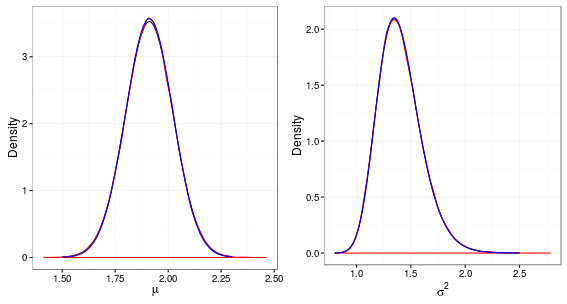
\includegraphics[width=0.7\linewidth,height=\textheight,keepaspectratio]{norminvg}
\caption{Marginal posterior densities for the model described in Section (\ref{sec:MCMC}). The true density is in black, the Monte Carlo sampler is red and the MFVB approximation is blue.}
\label{fig:norminvg}
\end{figure}

The set of mean field equations are only obtainable in the event that a prior that is conjugate to the model likelihood is used, restricting MFVB to exponential family models \citep{Beal2003}. In this case the optimal distributional family $q_i$ is the same as the prior, analagous to the relationship between a prior-posterior conjugate pair. 
In the event that a non-conjugate prior is used, the form of the distribution in (\ref{mf2}) is unrecognisable, a further approximation may be used by substituting in another distribution to replace the problematic $q_i(\theta_i |\boldsymbol{\lambda_i}).$ A common option is the use of a Gaussian distribution through either a Laplace approximation \citep{Friston2006} or a Delta Method inspired transform \citep{Wang2013}. This secondary level of approximation is analogous to the requirement of a Metropolis-Hastings-within-Gibbs step in MCMC to handle unrecognisable full conditional distributions.

\subsubsection{Stochastic Variational Bayes}

The requirement for an exponential family model without introducing further approximations, as well as restricting the approximating distribution to the factorisable family may be unsatisfactory in many applications. \citet{Paisley2012} and \citet{Ranganath2014} have adapted a gradient ascent algorithm for use in Variational Bayes, which selects optimal $\boldsymbol{\lambda}$ for a $q(\boldsymbol{\theta} | \boldsymbol{\lambda})$ from the class of distributions for which the score function can be evaluated, and the order of differentation of the ELBO with respect to $\boldsymbol{\lambda}$ and integration with respect to $\boldsymbol{\theta}$ are interchangable. The only model restriction is that the log likelihood for $y_{1:T}$ is able to be evaluated. We refer to the result as Stochastic Variational Bayes (SVB).

The application of gradient ascent in SVB iteratively takes the derivative of $\mathcal{L}(q(\boldsymbol{\theta} | \boldsymbol{\lambda}), y_{1:T})$ in (\ref{ELBO}) with respect to $\boldsymbol{\lambda}$ and the following updating step is applied until change in the ELBO is less than $\epsilon$.
\begin{equation}
\label{SVB1}
\boldsymbol{\lambda}^{(m+1)} = \boldsymbol{\lambda}^{(m)} + \rho^{(m)} \nabla_{\boldsymbol{\lambda}} \mathcal{L}(q(\boldsymbol{\theta} | \boldsymbol{\lambda}^{(m)}), y_{1:T}),
\end{equation}
where $\nabla_{\boldsymbol{\lambda}}\mathcal{L}(q(\boldsymbol{\theta} | \boldsymbol{\lambda}^{(m)}), y_{1:T})$ is the vector of partial derivatives of $\mathcal{L}(q(\boldsymbol{\theta} | \boldsymbol{\lambda}^{(m)}), y_{1:T})$ with respect to each element of $\boldsymbol{\lambda}$. This update requires some initial values $\boldsymbol{\lambda}^{(0)}$ and a sequence $\rho^{(m)}, m = 1, 2, \dots$ known as the learning rate. If $\rho^{(m)}$ is chosen to satisfy the following conditions the algorithm is guaranteed to converge to a local maximum \citep{Robbins1951}.
\begin{align}
&\sum_{m=1}^{\infty} \rho^{(m)} =  \infty \\
&\sum_{m=1}^{\infty} (\rho^{(m)})^2 <  \infty.
\end{align}

\citet{Ranganath2014} showed that a Monte Carlo estimate of the derivative of the ELBO can be given by
\begin{equation}
\label{SVB2}
\nabla_{\boldsymbol{\lambda}}\mathcal{L}(q(\boldsymbol{\theta} | \boldsymbol{\lambda}^{(m)}), y_{1:T}) \approx \frac{1}{S}\sum_{s=1}^{S} \nabla_{\boldsymbol{\lambda}} [\ln(q(\boldsymbol{\theta}_s | \boldsymbol{\lambda}^{(m)}))] (\ln (p(y_{1:T}, \boldsymbol{\theta}_s)) - \ln(q(\boldsymbol{\theta}_s | \boldsymbol{\lambda}^{(m)})))
\end{equation}
where $s = 1, \dots, S$ indicates simulations from $q(\boldsymbol{\theta} | \boldsymbol{\lambda}^{(m)})$.

\citet{Kingma2014} introduces the re-parameterisation trick, where an auxillary noise variable $\boldsymbol{\epsilon}$ and differentiable transformation $f(\cdot, \cdot)$ are introduced such that $\boldsymbol{\theta} = f(\boldsymbol{\epsilon}, \boldsymbol{\lambda}$. Examples include a location scale transformation from a standard normal $\epsilon$ or an inverse-CDF transformation from a uniform$(0, 1) \epsilon$. In this case (\ref{SVB2}) can be replaced with a lower variance estimator,
\begin{equation}
\label{reparameterise}
\nabla_{\boldsymbol{\lambda}}\mathcal{L}(q(\boldsymbol{\theta} | \boldsymbol{\lambda}^{(m)}), y_{1:T}) \approx \frac{1}{S}\sum_{s=1}^{S} \nabla_{\boldsymbol{\lambda}} \left( \ln (p(y_{1:T}, f(\boldsymbol{\epsilon}_s, \boldsymbol{\lambda}^{(m)})) - \ln(q(f(\boldsymbol{\epsilon}_s, \boldsymbol{\lambda}^{(m)})) \right)
\end{equation}
where $s = 1, \dots, S$ now indicates simulations from $q(\boldsymbol{\epsilon})$. This transformation removes the restriction that $q(\boldsymbol{\theta} | \boldsymbol{\lambda})$ belong to a distribution where the score function can be evaluated.

\citet{Duchi2011} developed the AdaGrad algorithm which can be implemented within SVB to control $\rho^{(m)}$. AdaGrad allows each $\lambda_i$ to have an independent $\rho^{(m)}_i$ that is inversely proportional to the gradient, so $\lambda$ takes bigger steps in flat regions and smaller steps in steep regions. 

Let 
\begin{equation}
\label{SVB3}
G_i^{(m)} = \sum_{j = 1}^{m} \left(\nabla_{\lambda_i}\mathcal{L}(q(\boldsymbol{\theta} | \boldsymbol{\lambda}^{(j)}), y_{1:T})\right)^2,
\end{equation}
then each component's learning rate is defined as
\begin{equation}
\label{SVB4}
\rho^{(m)}_i = \eta \left(G_i^{(m)}\right)^{-1/2}
\end{equation}
for some tuning parameter $\eta$.

The resulting Stochastic Gradient Ascent algorithm without reparameterisation proceeds below in Algorithm (\ref{alg:algorithm2}) with a $p$ dimensional $\boldsymbol{\lambda}$ vector.

\vspace{2mm}

\begin{algorithm}[H]
 \SetKwInOut{Input}{Input}
 \Input{Log Joint Density, Approximation family q}
 \KwResult{Variational Approximation}
 Initialise $\boldsymbol{\lambda}^{(1)}$\;
 Evaluate $\mathcal{L}(q(\boldsymbol{\theta} | \boldsymbol{\lambda}), y_{1:T})^{(1)}$ using $\boldsymbol{\lambda}^{(1)}$.\;
 \While{$\mathcal{L}(q(\boldsymbol{\theta} | \boldsymbol{\lambda}), y_{1:T})^{(m)} - \mathcal{L}(q(\boldsymbol{\theta} | \boldsymbol{\lambda}), y_{1:T})^{(m-1)} > \epsilon$}{
  Simulate $\boldsymbol{\theta}^s$ for $s = 1, \dots S$ from $q(\boldsymbol{\theta} | \boldsymbol{\lambda}^{(m)})$\;
  \For{$i =  1$ \KwTo $p$}{
      Calculate $\nabla_{\lambda_i}$ from (\ref{SVB2})\;
      Update $G_i^{(m)}$ and $\rho^{(m)}_i$ from (\ref{SVB3}) and (\ref{SVB4})\;
      }
  Update $\boldsymbol{\lambda}^{(m+1)}$ from (\ref{SVB1})\;
  Evaluate $\mathcal{L}(q(\boldsymbol{\theta} | \boldsymbol{\lambda}), y_{1:T})^{(m)}$\;
  Set $m = m + 1$\;
 }
 \caption{Stochastic Gradient Ascent for SVB}
  \label{alg:algorithm2}
\end{algorithm}

\subsubsection{Selection of the Approximating Distribution} \label{sec:selection}

Armed with an algorithm to find the Variational Bayes optimal parameters $\boldsymbol{\lambda}$ for a distribution $q$, there is a requirement to select a distribution $q$ that well approximates the true posterior. If reparameterised aproximating distribution is used to calculate the gradients in (\ref{reparameterise}) a function $f(\cdot, \cdot)$ that satisfies 

\begin{equation}
\label{optimalf}
f(\boldsymbol{\epsilon}, \boldsymbol{\lambda}) = p^{-1}(\boldsymbol{\epsilon})
\end{equation}

almost everywhere, where $\epsilon \sim U(0, 1)$ and $p^{-1}$ denotes the inverse CDF of the true posterior, will yield $q(\boldsymbol{\theta} | \boldsymbol{\lambda}) = p(\boldsymbol{\theta} | y_{1:T})$ and thus minimise the KL divergence. Attempts to model a suitably flexible function $f(\cdot, \cdot)$ include heirarchical models \citep{Ranganath2016a}, neural networks (\citealp{Kingma2014}; \citealp{Rezende2014}; \citealp{Rezende2015}; \citealp{Kingma2016}), and Gaussian processes \citep{Tran2016}.

These approaches introduce a large number of parameters that would considerably slow computation of updates, so we follow \citet{Tran2015} and use copulas to flexibly model approximations to the true posterior distribution. The copula modelling class provides a flexible way to construct these distributions, as it allows the dependence structure between parameters to be fit independently from the marginal distributions. \citet{Sklar1959} proves that any joint probability distribution can be written as the product of the marginals and a copula function,
\begin{equation}
\label{vc1}
p(\theta_1, \dots, \theta_k) = p(\theta_1) \dots p(\theta_k) c(P(\theta_1), \dots, P(\theta_k))
\end{equation}
where $p(\theta)$ is a pdf, $P(\theta)$ is a cdf, and $c(\cdot)$ is a copula. 

The flexibility of a copula is extended by the vine copula, a structure that permits the factorisation of a high-dimensional copula into a set of bivariate copulas, see \citet{Joe2014} and references within. A vine copula is represented by a series of trees, where the top-most tree is a graph that contains each variable as a node. The edges in each tree then form the nodes in the tree below, which are connected by an edge only if the associated edges in the previous tree shared the same node. This sequence is continued for a $k$ dimensional $\boldsymbol{\theta}$ until the $(k-1)'th$ tree is reached that contains only one edge. Each of the $k(k-1)/2$ edges represents a bivariate copula between the two unique parameters in the connected nodes, conditioned on every parameter appearing in both nodes. Refer to Figure (\ref{fig:vinecop}) for an example.
\vspace{3mm}
\begin{figure}[h]
\centering
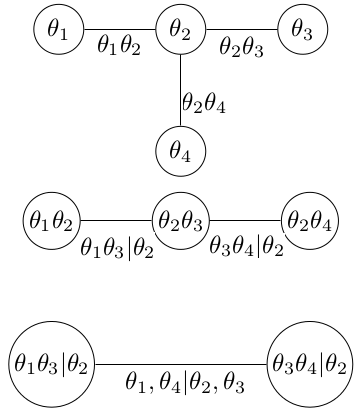
\includegraphics[width=0.4\linewidth,height=\textheight,keepaspectratio]{vines.png}
\vspace{2mm}
\caption{An example of a Vine Copula over four variables. The edges in the top tree represent unconditional bivariate copulas between the parameters on the connected nodes. The second tree edges represent the bivariate copulas for $\theta_1 \theta_3 | \theta_2$ and for $\theta_3 \theta_4 | \theta_2$, the conditioning on $\theta_2$ caused by its appearance in each connected node. The edge in the final tree represents the bivariate copula for $\theta_1, \theta_4 | \theta_2, \theta_3$, as both $\theta_2$ and $\theta_3$ appear in the connected nodes.}
\label{fig:vinecop}
\end{figure}


The flexibility in selecting a factorisation and set of bivariate copula familys in vine copula greatly increases the ability to model dependency in a distribution, but the cardinality of the set of possible vine structures and choices of family for each bivariate copula grows factorially with the number of parameters, so without detailed problem specific information the application of a vine copula to Stochastic Variational Bayes is difficult. 

Given a sample of $\boldsymbol{\theta}$, Di{\ss}mann's algorithm \citep{Dissmann2013} can be used to select the best vine factorisation by selecting a maximum spanning tree for the first tree that maximises the sum of Kendall's Tau for each pair of nodes connected by an edge. The algorithm then selects the best family for each of the first tree's bivariate copula by minimising an information criterion such as AIC. Edges and copula families in subsequent trees are selected sequentially. In the real-time forecasting models used for electricity load demand, MCMC samples of the posterior distribution are available, though often immediately out of date. The approach used in this thesis is to run an MCMC algorithm, thin the resulting draws until they are effectively independent, choose an optimal family for each marginal distribution by AIC, then run Di{\ss}mann's algorithm to infer a vine copula structure that fits the data well. This vine copula is used to construct an approximating distribution $q(\boldsymbol{\theta} | \boldsymbol{\lambda})$ that can then be used in an SVB algorithm to update $q(\boldsymbol{\theta} | \boldsymbol{\lambda})$ as more observations become available. MCMC can be ran simultaneously and the resulting sample can be used to check if the distribution $q$ should be changed. 

\subsection{Time Series Application}

In this section the techniques described throughout Section \ref{sec:BayesInf} are applied to a simple, but widely used, time-series model. 
Consider the second order auto-regressive time series model, denoted by AR(2) and described by 
\begin{equation}
\label{AR2}
y_t = \phi_1 y_{t-1} + \phi_2 y_{t-2} + \epsilon_t
\end{equation}
where $\epsilon_t \sim \mathcal{N}(0, \sigma^2)$ for $t = 3, \dots, T$. The first two observations, $y_1$ and $y_2$ are distributed according to 
\begin{equation}
\label{AR2initial}
y_1, y_2, \sim \mathcal{N}(\boldsymbol{0}, \Sigma)
\end{equation}
where 
\begin{align}
\Sigma &= \left[ \begin{array}{cc} \gamma(0) & \gamma(1) \\ \gamma(1) & \gamma(0) \end{array} \right] \nonumber \\
\gamma(0) &= \sigma^2 \frac{1-\phi_2}{(1+\phi_2)((1-\phi_2)^2 - \phi_1^2)} \nonumber \\
\gamma(1) &= \sigma^2 \frac{\phi_1}{(1+\phi_2)((1-\phi_2)^2 - \phi_1^2)} \nonumber.
\end{align}

The likelihood of parameters $\boldsymbol{\theta} = (\phi_1, \phi_2, \sigma^2)'$, that is, the density of the observations $y_{1:T}$, given $\boldsymbol{\theta}$, viewed as a function of $\boldsymbol{\theta}$, is given by
\begin{align}
\label{likelihood}
L(\theta | y_{1:T}) &= p(y_1, y_2 | \theta) \prod_{t=3}^{T}p(y_t | y_{1:t-1}, \theta) \nonumber \\
&\propto |\Sigma|^{-1/2} \sigma^{-(T-2)} \exp \left\{ \frac{-1}{2} (y_1, y_2) \Sigma^{-1} (y_1, y_2)' \right\} \nonumber \\
&\times \exp \left\{ \frac{-1}{2\sigma^2} \left( \sum_{t=3}^{T}(y_t - \phi_1 y_{t-1} - \phi_2 y_{t-2})^2 \right) \right\}.
\end{align}

We assume that the prior distribution, is given by
\begin{equation}
p(\sigma^2, \phi_1, \phi_2) \propto \sigma^{-2} \mathbb{I}(\phi_2 > -1)\mathbb{I}(\phi_2 < 1 + \phi_1) \mathbb{I}(\phi_2 < 1 - \phi_1), 
\label{ar2prior}
\end{equation}
where $\mathbb{I}$ is the indicator function that equals one if the condition in the brackets is true and zero otherwise. This prior has positive mass if and only if a pair $(\phi_1, \phi_2)$ is within the AR(2) stationary region. Note that this prior is not conjugate due to the form of $\phi_1$ and $\phi_2$ in $\Sigma$, and thus MFVB cannot be applied. Upon examination of the form of the product of the likelihood function in (\ref{likelihood}) and the prior density in (\ref{ar2prior}) it can be seen that the full conditional distribution $p(\sigma^2 | y, \phi_1, \phi_2)$ is an Inverse Gamma distribution, while the conditionals for both $\phi$ parameters are intractable but can be sampled using a Metropolis-Hastings step with truncated bivariate normal random walk proposal distribution. The truncation ensures that draws of $(\phi_1,\phi_2)$ are only taken from the AR(2) stationary region. 

Data was simulated with $T = 150, \sigma^2 = 1, \phi_1 = 0.7$ and $\phi_2 = 0.2$, then the MCMC algorithm described above is applied. Marginal distributions are fit to each parameter in $\boldsymbol{\theta}$ by minimising AIC, and an application of Di{\ss}mann's algorithm to the draws found an optimal Vine Copula structure. The functional form of $q(\boldsymbol{\theta} | \boldsymbol{\lambda})$ to be used in SVB is:
\begin{itemize}
\item $q(\phi_1 | \boldsymbol{\lambda}_1)$ - Gaussian marginal
\item $q(\phi_2| \boldsymbol{\lambda}_2)$ - Gaussian marginal
\item $q(\sigma^2| \boldsymbol{\lambda}_3)$ - Inverse Gamma marginal
\item $c(Q(\phi_1), Q(\phi_2) | \boldsymbol{\lambda}_4)$ - Gaussian copula
\item $c(Q(\phi_1), Q(\sigma^2))$ - Independent
\item $c(Q(\phi_2), Q(\sigma^2) | Q(\phi_1))$ - Independent
\end{itemize}

Figure \ref{fig:VBfit} displays the marginal and bivariate posterior distributions that result from each of the Stochastic Variational Bayes (blue) and the MCMC (red) approaches. In the case of MCMC, a kernel estimate obtained from the relevant posterior sample is displayed, whereas for SVB the form of the relevant vine copula marginal determines the shape of the marginal posterior. As is clear from the figure, SVB appears to have selected values for $\boldsymbol{\lambda}$ that closely match the MCMC posterior distribution. SVB required approximately one hundredth of the computation time required for MCMC.

\begin{figure}[h]
\centering
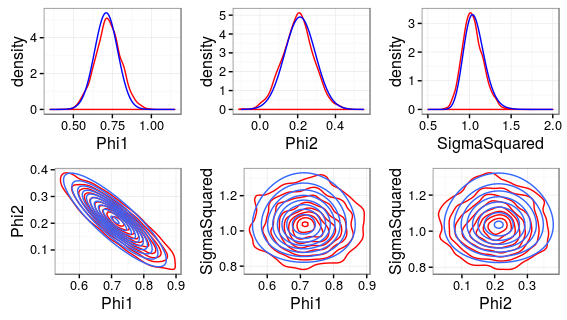
\includegraphics[width=0.7\linewidth,height=\textheight,keepaspectratio]{VBfit.png}
\caption{The fit of an SVB algorithm (blue) compared to MCMC (red) for the AR(2) model.}
\label{fig:VBfit}
\end{figure}

\section{Electricity Load Forecasts} \label{sec:ElecLoad}
\subsection{Motivation}

The literature for electricity forecasting for both load and price is wide, and contains models based on many different fields, such as game theory, time-series modelling and neural networks, see \citet{Weron2014} for a recent review. Density forecasting for short term electricity load has had less attention, with \citet{Fan2012} and \citet{He2016} being notable examples, which used bootstrapping and quantile regression respectively to generate forecast densities. Both of these approaches create forecast densities that are conditioned on the model and estimated parameters being correct, while the Bayesian approach used in this thesis can average over parameter and model uncertainty leading to a more accurate forecast density. This thesis also aims to re-estimate the model after each data point is observed to fully take advantage of any extra information on changes in parameters and thus further increase the accuracy of the forecast density. 

Half hourly electricity load data for Victoria, Australia is provided by the Australian Energy Market Operator (AEMO) for the 2011-2015 period, and is plotted in Figure \ref{fig:loadplot}. The time series displays strong seasonal characteristics, with time of year, day of week, and time of day patterns. This yearly pattern is characterised by a low median load with high volatility in summer and a more consistent curve in winter. Electricity load is strongly dependent on temperature, with high load experienced on both very cold and very hot days. In summer periods, load is often low but shows extreme volatility, while load slowly rises then falls in winter and displays significantly less volatility. 

The wholesale electricity market in Victoria operates by market participants sending electricity bid and offers for each five minute period to AEMO, which then matches electricity generators with retailers to determine the dispatch load and associated price. At the end of each half-hour block the previous six five-minute dispatch prices are averaged to obtain the final spot price that participants trade at. Market participants are allowed to revise bids and offers at any point before dispatch. The electricity supply curve is strongly hockey stick shaped, as renewables and coal generators are able to provide a large load cheaply but if demand exceeds this level the price spikes as other generators must be brought online expensively. These characteristics of the electricity market leads to a large amount of volatility in prices demonstrated by Figure \ref{fig:rrpplot}. The seasonal effects of the load data are also present in prices, but these effects are dominated by irregular spikes as high as \$9,974/mWh, compared to a four year mean price of \$42/mWh.

\begin{figure}[h]
\centering
\includegraphics[width=\linewidth,height=\textheight,keepaspectratio]{load_timeseries.png}
\caption{Half hourly load data measured in megawatt hours for Victoria from January 1 2011 to December 31 2015.}
\label{fig:loadplot}
\end{figure}

\begin{figure}[h]
\centering
\includegraphics[width=\linewidth,height=\textheight,keepaspectratio]{RRP_timeseries.png}
\caption{Half hourly price data for Victoria from January 1 2011 to December 31 2015.}
\label{fig:rrpplot}
\end{figure}

\subsection{Exponential Smoothing}

\citet{Taylor2003} explores the seasonal properties of minute-by-minute electricity demand in the United Kingdom and introduces the double seasonal Holt-Winters exponential smoothing model with daily and weekly effects described by (\ref{ds-hw1})-(\ref{ds-hw4}). Yearly seasonal effects are omitted as their inclusion requires a large number of latent states to be estimated, however \citet{Taylor2008} later provides empirical support that this model is superior to other common time-series models such as SARIMA based models that include a yearly seasonal effect. The double seasonal Holt-Winters exponential smoothing model is described by
\begin{align}
y_t &= l_{t-1} + d_{t-m_1} + w_{t-m_2} + e_t \label{ds-hw1} \\
l_t &= \alpha (y_t - d_{t-m_1} - w_{t-m_2}) + (1 - \alpha)l_{t-1} \label{ds-hw2}\\
d_t &= \delta (y_t - l_{t-1} - w_{t-m_2}) + (1 - \delta)d_{t-m_1} \label{ds-hw3} \\
w_t &= \omega (y_t - l_{t-1} - d_{t-m_1}) + (1 - \omega)w_{t-m_2} \label{ds-hw4}
\end{align}
where $m_1$ and $m_2$ are the lengths of the daily and weekly cycle, and the smoothing parameters $\alpha, \delta, \omega$ are also restricted to to lie in $(0, 1)^3$. This can be rewritten as a single source of error state-space model \citep{Snyder1985},

\begin{align}
y_t &= l_{t-1} + d_{t-m_1} + w_{t-m_2} + e_t \label{ds-hw-ssoe1} \\
l_t &= l_{t-1} + \alpha e_t \label{ds-hw-ssoe2} \\
d_t &= d_{t-m_1} + \delta e_t \label{ds-hw-ssoe3} \\
w_t &= w_{t-m_2} + \omega e_t \label{ds-hw-ssoe4}. 
\end{align}
The unknown parameters are $\boldsymbol{\theta} = (\alpha, \delta, \omega)', \sigma^2$ and $\textbf{b}_0 = (l_0, d_0, \dots, d_{-(m_1 - 1)}, w_0, \dots, w_{-(m_2 - 1)})'$ a $k = m_1 + m_2 + 1$ length vector of the initial states of the latent variables. The single source of error state-space model refers to the random error $e_t$ being shared across the data each latent variable, and allows the likelihood to be expressed as a closed form function of the unknown parameters.

\citet{Forbes2000} provides a transformation to the model that allows a straight-forward Bayesian analysis in small samples, noting that the state space model can be expressed as
\begin{align}
y_t &= \textbf{x}' \textbf{b}_t + e_t \label{ss_me} \\
\textbf{b}_t &= T \textbf{b}_{t-1} + \tilde{\boldsymbol{\theta}} e_{t-1} \label{ss_te}.
\end{align}

Using $D = T - \tilde{\boldsymbol{\theta}} \textbf{x}'$, the transition equation in (\ref{ss_te}) can be written as 
\begin{equation}
\textbf{b}_t = D \textbf{b}_{t-1} + \tilde{\boldsymbol{\theta}} y_t \label{ss_te_2}.
\end{equation}

Setting $\bar{\textbf{b}}_0 = 0$, the recursion in (\ref{ss_te_2}) allows the transformed observations $\tilde{y}_t$ to be obtained via
\begin{equation}
\tilde{y}_t = y_t - x'\bar{\textbf{b}}_{t-1} \label{ss_rp_y}.
\end{equation}

Furthermore, transformed regression variables $\tilde{\textbf{x}}_t$ can be obtained from $\tilde{\textbf{x}}_t = D\tilde{\textbf{x}}_{t-1}$ with $\tilde{\textbf{x}}_0 = \textbf{x}$. Collecting these as $\widetilde{X}' = (\tilde{\textbf{x}}_1, \tilde{\textbf{x}}_2, \dots, \tilde{\textbf{x}}_T)$ and $\widetilde{Y}' = (\tilde{y}_1, \tilde{y}_2, \dots, \tilde{y}_T)$, and assuming the errors $e_t$ are Gaussian, the model likelihood is
\begin{equation}
L(\boldsymbol{\theta}, \sigma^2, \boldsymbol{b}_0 | y_{1:T}) \propto \sigma^{-T} \exp \left\{ \frac{-1}{2\sigma^2}(\widetilde{Y} - \widetilde{X}\boldsymbol{b}_0)'(\widetilde{Y} - \widetilde{X}\boldsymbol{b}_0) \right\}.
\end{equation}
Hence once conditioned on a draw of $\boldsymbol{\theta}$, the remaining unknown parameters can be sampled as a Bayesian linear regression problem.

\citet{Forbes2000} provides the marginal distribution of $\boldsymbol{\theta}$,
\begin{equation}
\label{exp-sm-marginal}
p(\boldsymbol{\theta} | y_{1:T}) \propto \left| \widetilde{X}' \widetilde{X} \right|^{-1/2} \tilde{s}^{-(T-k)} p(\boldsymbol{\theta}),
\end{equation}
where $\tilde{s}^2 = (\widetilde{Y} - \widetilde{X}\hat{\textbf{b}}_0)'(\widetilde{Y} - \widetilde{X}\hat{\textbf{b}}_0) / (T - (m_1 + m_2 + 1))$ is the sum of squared errors for $\hat{\textbf{b}}_0 = (\widetilde{X}'\widetilde{X})^{-1}\widetilde{X}'\widetilde{Y}$.
With the seasonality parameterisation in (\ref{ds-hw-ssoe1}) - (\ref{ds-hw-ssoe4}), the matrix $\widetilde{X}' \widetilde{X}$ is singular, but restricting the latent variables via
\begin{align}
d_t &= - \sum_{i=1}^{m_1-1} d_{t-i} \\
w_t &= - \sum_{i=1}^{m_2-1} w_{t-i}
\end{align}
avoids this problem. The resulting model is described by
\begin{align}
y_t &= l_{t-1} - \sum_{i = 1}^{m_1 - 1}d_{t-i} - \sum_{i = 1}^{m_2 - 1}w_{t-i} + e_t \label{ds-hw-rp1} \\
l_t &= l_{t-1} + \alpha e_t \label{ds-hw-rp2} \\
d_t &= - \sum_{i = 1}^{m_1 - 1}d_{t-i} + \delta e_t \label{ds-hw-rp3} \\
w_t &= - \sum_{i = 1}^{m_2 - 1}w_{t-i} + \omega e_t \label{ds-hw-rp4}.
\end{align}
and $\textbf{b}_0 = (l_0, d_0, \dots, d_{-(m_1 - 2)}, w_, \dots, w_{-(m_2 - 2)})'$ is a length $k = m_1 + m_2 - 1$ vector.

\citet{Forbes2000} recommends numerical integration of the marginal posterior density of $\boldsymbol{\theta}$ in (\ref{exp-sm-marginal}), however the problems with using this method in our model are two-fold: repeating a three dimensional numerical integration each time a new data point is observed within the five minute window is not feasible, and the $T$ in the exponent makes most evaluations of $p(\boldsymbol{\theta}  | y_{1:T})$ computationally zero when $T$ is large, as is the case with high frequency electricity load data. An efficient MCMC algorithm that scales to large datasets with models using multiple seasonality parameters will be required to sample the full posterior distribution $p(\boldsymbol{\theta} , \sigma^2, b_0 | y_{1:T})$ and obtain an approximating distribution $q(\boldsymbol{\theta}, \sigma^2, b_0 | \boldsymbol{\lambda})$ with a reasonable goodness of fit. From this point, Stochastic Variational Bayes will be find an approximation to the updated posterior distribution as more data is observed, and provide the predictive density $q(y_{T+J+1} | y_{T+J})$.

\section{Discussion} \label{sec:Discussion}

One of the major aims of this thesis is to provide a methodology to forecast predictive densities with minimal calculation required to update parameter estimates as more data is observed, so an accurate forecast can be made even on a very short time-frame. However the short time-frame and high frequency of observating data implies that there is already a large number of past observations available, so any the marginal information from an additional observation on the parameters may be minimal. 

The benefits of rapidly updating parameters will be increased in situations where there are major changes in the data generating process over time. One example is a state-space model where information on the next latent state is increased significantly after observing the most recent data point. However, unless the model has either a non-linearity or non-Gaussian error, the Kalman filter can be applied to obtain an accurate predictive density without difficult computation. Volatility forecasting for stock returns is a potentially useful application as data is observed on a short time-frame, and the stochastic volatility state-space models commonly used do not admit the use of the Kalman filter. 

A contribution of this thesis is the use of information generated by MCMC to develop a Vine Copula used by the approximating distribution in Stochastic Variational Bayes, but updating state-space models by SVB requires an approximation for latent states associated with newly observed data that have not been included in the most recent MCMC sample. In this case, the dependence for the new latent state must be extrapolated from the copula structure used for previous latent states, which may be sub-optimal. The robustness of SVB approximations to choices of $q$ that badly fit the true posterior should be investigated. Development of the theory of choosing the distribution $q$ is currently extremely active, a methodology that relies on the form of the model likelihood and prior rather than MCMC samples to determine the form of a well-fitting approximation would be of interest. 

Finally, there is a trade-off between the predictive accuracy of MCMC and the ability to update Variational Bayes posterior distributions. The statistical error associated with using an approximate distribution has not been investigated in the literature and we shall contribute by comparing this error in forecasting with VB to the statistical error associated with forecasting based on an MCMC generated posterior distribution that is not conditioned on the most recent data.

\section{Timeline} \label{sec:Timeline}

\begin{tabular}{|l|l|}
\hline
  June 2017 & $\cdot$ Derive an efficient MCMC algorithm for exponential smoothing and \\
  & apply SVB for electricity load forecasting. \\
  & $\cdot$ Similarly apply SVB to competing models such as SARIMA. \\
  & $\cdot$ Compare forecast accuracy to MCMC with and without updates to \\
  & parameters. \\ \hline
  December 2017 & $\cdot$ Investigate state-space models, including time-varying parameters, \\
  & non-linearities or non-Gaussian errors. \\
  & $\cdot$ Apply this to Stochastic Volatility models. \\
  & $\cdot$ Extend model with multivariate data and Markov Switching mechanisms.\\
  & $\cdot$ Compare results to Particle Filter based methods. \\  \hline
  June 2018 & $\cdot$Investigate impact of sub-optimal approximating distributions  \\
  & such as mis-specified copulas for new latent states. \\
  & $\cdot$ Investigate other ways to construct the approximating distribution  \\
  & either with or without a posterior sample being available. \\  \hline
  December 2018 & $\cdot$ Allow extra time for updates in the active VB literature  \\
  & to develop, and adapt them to the benefit my research. \\  \hline
  May 2019 & $\cdot$ Put separate parts together and polish the final thesis for submission. \\
\hline
\end{tabular}

\bibliographystyle{asa}
\bibliography{references}

\end{document}
\grid
\grid
\grid
\grid
\grid
\grid
\grid
